\documentclass[12pt]{article}
\usepackage[utf8]{inputenc}
\usepackage{amsmath}
\usepackage{subcaption}
\usepackage{float}
\usepackage{graphicx}
\usepackage{epstopdf}
\usepackage{color}
\newcommand{\de}[1]{$\langle${{\color{cyan}\slshape{\bfseries DE:} #1}$\rangle$}}
\newcommand{\rz}[1]{$\langle${{\color{magenta}\slshape{\bfseries RZ:} #1}$\rangle$}}

\setlength{\parindent}{4em}
\setlength{\parskip}{1em}
\renewcommand{\baselinestretch}{1.5}

\title{Intensional infect proportion of susceptible}

\begin{document}
\maketitle

\de{There is some rate at which susceptibles are intentionally infected, say $r$, so there is a term $-rS$ in the dimensional SIR equations.  We are expressing the SIR model in dimenionless form, so let $\eta=r/(\gamma+\mu)$ and then we get the following.}

Here is the system we are investigating:
\begin{align}
\frac{\mathrm{d}S}{\mathrm{d}\tau}&=\epsilon -\mathcal{R}_0 SI-\eta S-\epsilon S\\
\frac{\mathrm{d}I}{\mathrm{d}\tau}&=\eta S+\mathcal{R}_0 SI-I\\
\frac{\mathrm{d}R}{\mathrm{d}\tau}&=(1-\epsilon)I-\epsilon R
\end{align}

Here $\gamma$ is mean infectious period, $\mu$ is birth/death rate, $r$ is rate of intensional infection. $\epsilon=\frac{\mu}{\gamma+\mu}$, $\mathcal{R}_0$ is the basic reproduction number.

Since last time we discussed that, it is not very meaningful to divide $I$ into $I_T$ and $I_N$. Thus, I just used I this time to investigate the system's equilibrium, stability and other properties.
\section{EE}
Endemic equilibrium is the following:

\begin{align}
I &= \frac{-(\eta+\epsilon-\epsilon\mathcal{R}_0)+\sqrt{(\eta+\epsilon-\epsilon\mathcal{R}_0)^2+4\mathcal{R}_0\epsilon \eta}}{2\mathcal{R}_0}\\
S &= \frac{1}{\mathcal{R}_0}-\frac{2\eta}{\mathcal{R}_0(-(\eta+\epsilon-\epsilon\mathcal{R}_0)+\sqrt{(\eta+\epsilon-\epsilon\mathcal{R}_0)^2+4\mathcal{R}_0\epsilon \eta}+2\eta)}
\end{align}

Jacobian is the following.
\begin{equation}
\mathcal{J} =
\begin{bmatrix}
    \ -\mathcal{R}_0 I-\eta-\epsilon       & -\mathcal{R}_0 S \\
    \ \eta+\mathcal{R}_0 I       & \mathcal{R}_0 S-1 \\
\end{bmatrix}
\end{equation}

Again, for simplicity. Let $G=-(\eta+\epsilon-\epsilon\mathcal{R}_0)+\sqrt{(\eta+\epsilon-\epsilon\mathcal{R}_0)^2+4\mathcal{R}_0\epsilon \eta}$. Notice, $G>0$, if $\epsilon,\eta\neq 0$

So Jacobian at E.E. is:

\begin{equation}
\mathcal{J} =
\begin{bmatrix}
    \ \frac{G}{2}-\eta-\epsilon       & -1+\frac{2\eta}{G+2\eta} \\
    \ \eta+\frac{G}{2}       & -\frac{2\eta}{G+2\eta} \\
\end{bmatrix}
\end{equation}

Thus, eigenvalues of of Jacobian are the following:

\begin{align}
\lambda_{1,2} &= \frac{-(G^2+4\eta G+2\epsilon G+4\eta^2+4\epsilon\eta+4\eta) }{4(G+2\eta)}\\
& \pm \frac{\sqrt{((G^2+4\eta G+2\epsilon G+4\eta^2+4\epsilon\eta+4\eta)^2-4(2G^3+12\eta G^2+24\eta^2 G+8\epsilon\eta G+16\eta^3+16\epsilon\eta^2)}}{4(G+2\eta)}
\end{align}

Since $G,\eta >0$, we can conclude that Re($\lambda$)$<0$, thus E.E. is stable.

Now we are interested in equation (9), if the discriminant is positive/negative. Which could indicate whether there is a damped oscillation.

Now we want to analyze with specific values of each parameter.

A reasonable choice would be using smallpox, considering its background of intensional infection in human history.


\subsection{Take $\epsilon$ to be the variable}
The following values are used: $\mu=\frac{1}{50*365}$, $\gamma=\frac{1}{22}$, $\mathcal{R}_0=4.5$. Also, $\epsilon=\frac{\mu}{\mu+\gamma}=0.0012$

So now, $G=-(\eta-0.0042)+\sqrt{(\eta-0.0042)^2+0.0216\eta}$

\begin{align}
\lambda_{1,2} &= \frac{-(G^2+4\eta G+0.0024 G+4\eta^2+0.0048\eta+4\eta) }{4(G+2\eta)}\\
& \pm \frac{\sqrt{((G^2+4\eta G+0.0024 G+4\eta^2+0.0048\eta+4\eta))^2-4(2G^3+12\eta G^2+24\eta^2 G+0.0096\eta G+16\eta^3+0.0192\eta^2)}}{4(G+2\eta)}
\end{align}

So I plotted the discriminant using Mathematica, here is what I got:

\begin{figure}[h!]
  \caption{Plot discriminant with $\eta$ to be the variable.}
  \centering
  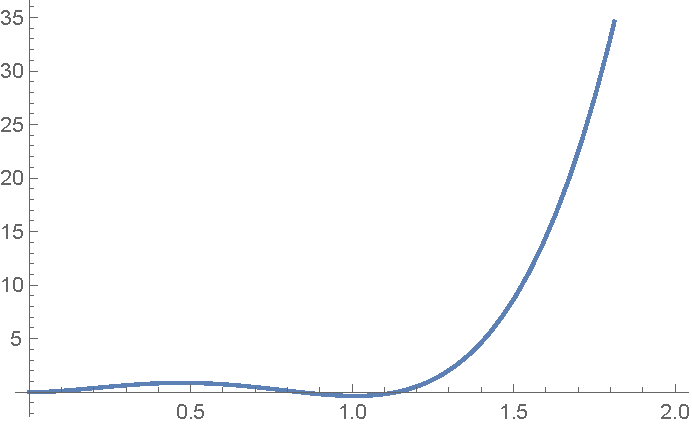
\includegraphics[width=1\textwidth]{Figures/Discriminant_plot_S.pdf}
\end{figure}

The $\eta$-intercept of this plot is $\eta_1=0.000704619$, $\eta_2=0.840164$, $\eta_3=1.13557$. The corresponding interpretations are: average time before being intentional infected are 31184.95, 26.15, 19.35 days, respectively.

Realistically, it should not take 85 years to intentionally infect an individual. so we can reject $\eta_1=0.000704619$.

Thus, if we are intentionally infecting slower than $\eta_2$ or faster than $\eta_3$, there is no damped oscillation, or otherwise there is.

For value of $\eta$, it is reasonable to assume the average number of days before an individual to be intentionally infected is between 30-60 days. Thus our range of $\eta$ could vary from 0.36623 - 0.73245. Thus, from this range, we should get a positive discriminant value, hence, there is no damped oscillation.

\subsection{Take $\mathcal{R}_0$ as variable}

This time, I again take $\mu=\frac{1}{80*365}$, $\gamma=\frac{1}{22}$, $\epsilon=\frac{\mu}{\mu+\gamma}=0.000753$. 

Now I take $\eta=0.4885$, as it correspond to the average number of days before an individual get intentionally infected being 45 days.

Again, I did the plot of discriminant.

\begin{figure}
  \caption{Plot discriminant with $\mathcal{R}_0$ to be the variable.}
  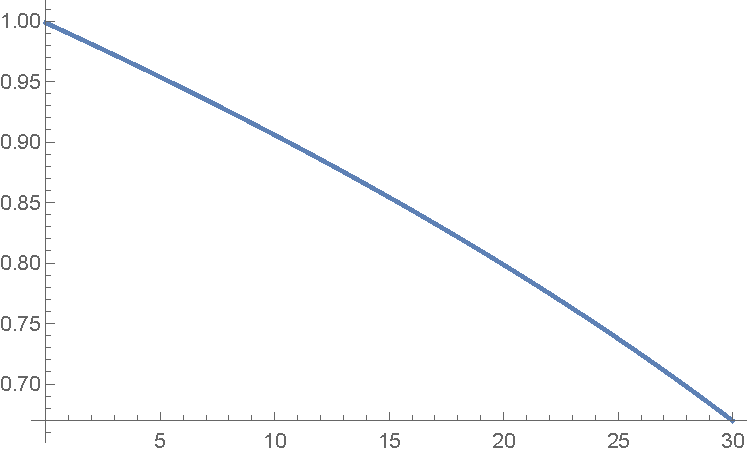
\includegraphics[width=1\textwidth]{Figures/Plot_R_S.pdf}
\end{figure}

The plotting result shows that discriminant is always positive,for a reasonable $\mathcal{R}_0$ value. Thus, if we take $\eta=0.4885$, there is never going to be a damped oscillation.

The value of discriminant is much more sensitive to $\eta$ than to $\mathcal{R}_0$.

\section{DFE}

Disease free equilibrium is the equilibrium when there is nobody infected in the system, which means, $I=0$

Thus we have $\frac{\mathrm{d}I}{\mathrm{d}\tau}=\eta S+\mathcal{R}_0 SI-I=\eta S=0$

In our case, there is no DFE. When $I=0$, we are still intensionally infecting susceptible,  therefore, there is no equilibrium in which $I=0$.

\end{document}